\chapter{Diagrama de paquetes}
Para el desarrollo de la aplicación se han hecho uso de un conjunto de archivos, organizados en distintos paquetes, los cuales se 
irán definiendo a continuación.\\

Las clases se agruparán mediante el empleo de paquetes que se organizarán mostrando sus relaciones de importación/exportación en un
diagrama de paquetes. Los diagramas de paquetes se usan para representar relaciones lógicas entre distintos elementos como pueden ser
clases y casos de usos, que mantienen una relación semántica entre ellos. \\

   \section{Identificación de paquetes}
   \begin{figure} [H] \begin{center}
   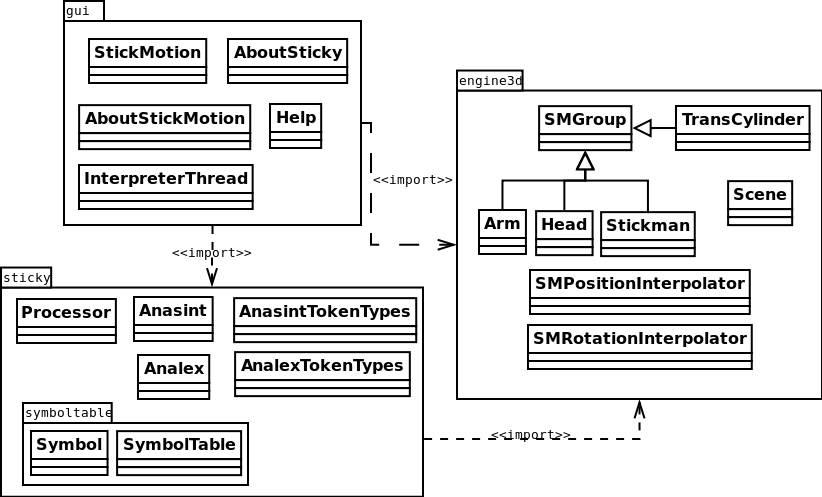
\includegraphics[width=0.7\textwidth]{./imagenes/paquetes}\label{DiagramaPaquetes}
   \caption{Diagrama de paquetes de \textbf{\textit{StickMotion}}.}
   \end{center} \end{figure}
   Se empaquetarán las clases agrupándolas en los siguientes paquetes, correspondiendose con los componentes funcionales en los que se
   descompuso el sistema en el análisis de requisitos. \\

   En la figura \ref{DiagramaPaquetes} se muestra el diagrama indicando las relaciones de importación que se realizan entre los distintos
   paquetes. \\


   \section{Paquete engine3d}
   Este paquete contendrá todo el código relacionado con las animaciones 3D. Incluye las siguientes clases:
   \begin{itemize}
      \item SMGroup.
      \item TransCylinder.java
      \item Arm.java
      \item Head.java
      \item Stickman.java
      \item Scene.java
      \item SMPositionInterpolator.java
      \item SMRotationInterpolator.java
   \end{itemize}


   \section{Paquete gui}
   Este paquete contendrá todo el código relacionado con la interfaz gráfica. Incluye las siguientes clases:
   \begin{itemize}
      \item StickMotion.java
      \item AboutSticky.java
      \item AboutStickMotion.java
      \item Help.java
      \item InterpreterThread.java
   \end{itemize}


   \section{Paquete sticky}
   Este paquete contendrá el código relacionado con ANTLR, y en general, con los tres analizadores. Contiene las siguientes clases:
   \begin{itemize}
      \item Processor.java
      \item analex.g
      \item Analex.java
      \item AnalexTokenTypes.java 
      \item Analex.smap 
      \item AnalexTokenTypes.txt
      \item anasint.g 
      \item Anasint.java 
      \item AnasintTokenTypes.java 
      \item Anasint.smap
      \item AnasintTokenTypes.txt
      \item Asímismo existe también otro paquete, \textbf{\textit{symboltable}}, cuyo contenido es:
            \begin{itemize}
               \item Symbol.java
               \item SymbolTable.java
            \end{itemize}
   \end{itemize}



